% --------------------------------------
% Document Class
% --------------------------------------
\documentclass[a4paper,11pt]{article}
% --------------------------------------



% --------------------------------------
% Use Package
% --------------------------------------


\usepackage[francais]{babel}
%\usepackage{ucs}
\usepackage[utf8]{inputenc}
\usepackage[T1]{fontenc}

\usepackage{makeidx}
\usepackage{color}
\usepackage{graphicx}
\usepackage{float}
\usepackage[hidelinks]{hyperref} 
\usepackage{geometry}
%\usepackage{lastpage}
%\usepackage{marginnote}
\usepackage{fancyhdr}
%\usepackage{titlesec}
%\usepackage{framed}
\usepackage{amsmath}
\usepackage{empheq}
\usepackage{array}
\usepackage{multicol}
%\usepackage{adjustbox}

% insert code
\usepackage{listings}

% define our color
\usepackage{xcolor}

% code color
\definecolor{ligthyellow}{RGB}{250,247,220}
\definecolor{darkblue}{RGB}{5,10,85}
\definecolor{ligthblue}{RGB}{1,147,128}
\definecolor{darkgreen}{RGB}{8,120,51}
\definecolor{darkred}{RGB}{160,0,0}

% other color
\definecolor{ivi}{RGB}{141,107,185}


\lstset{
    language=Scilab,
    captionpos=b,
    extendedchars=true,
    frame=lines,
    numbers=left,
    numberstyle=\tiny,
    numbersep=5pt,
    keepspaces=true,
    breaklines=true,
    showspaces=false,
    showstringspaces=false,
    breakatwhitespace=false,
    stepnumber=1,
    showtabs=false,
    tabsize=3,
    basicstyle=\small\ttfamily,
    backgroundcolor=\color{ligthyellow},
    keywordstyle=\color{ligthblue},
    morekeywords={include, printf, uchar},
    identifierstyle=\color{darkblue},
    commentstyle=\color{darkgreen},
    stringstyle=\color{darkred},
}


% --------------------------------------



% --------------------------------------
% Page setting
% --------------------------------------
%\pagestyle{empty}
\setlength{\headheight}{15pt}

\setcounter{secnumdepth}{3}
\setcounter{tocdepth}{2}

\makeatletter
\@addtoreset{chapter}{part}
\makeatother 

\hypersetup{         % parametrage des hyperliens
  colorlinks=true,      % colorise les liens
  breaklinks=true,      % permet les retours à la ligne pour les liens trop longs
  urlcolor= blue,       % couleur des hyperliens
  linkcolor= black,     % couleur des liens internes aux documents (index, figures, tableaux, equations,...)
  citecolor= green      % couleur des liens vers les references bibliographiques
}

% --------------------------------------

% --------------------------------------
% Information
% --------------------------------------
\title{Compte-rendu TP4 TI : Transformation ponctuelle}
\author{Elliot VANEGUE et Gaëtan DEFLANDRE}
% --------------------------------------

\definecolor{myColor}{rgb}{0.5, 0.1, 0.75}

% --------------------------------------
% Begin content
% --------------------------------------
\begin{document}

% Set language to english
  \selectlanguage{francais}

  % Start the page counting
  \pagenumbering{arabic}

  \maketitle
  
  \mbox{}
  \newpage
  \clearpage
  
  \section*{Introduction}
  Lors de ce TP, nous avons travaillé avec l'outil ImageJ dans le but d'utiliser et de comprendre
  le fonctionnement de l'histogramme de niveaux de gris. Pour cela, nous avons effectué des exercices 
  sur le changement de la dynamique de gris en utilisant des LUT\footnote{Look Up Table}.

  \section{Extension de l'histogramme de niveau de gris}
  Pour commencer, nous avons écris une macro permettant de récupérer les niveaux de gris minimum et 
  maximum d'une image dans le but de les modifier afin d'avoir une dynamique de gris allant de 
  0 à 255. Pour cela nous avons appliqué la transformation linéaire suivante : 
  \begin{align*}
   round\left(\frac{255 * pixel(i,j) - min}{max - min}\right)
  \end{align*}

  Dans cette formule, la fonction round permet d'arrondir le résultat à l'entier le plus proche.
  En effectuant ce calcul sur chaque pixel, nous obtenons les résultat suivant :\\
  
  \begin{tabular}{|c|c|c|c|}
   \hline
   image départ & histogramme & image étendue & histogramme\\
   \hline
   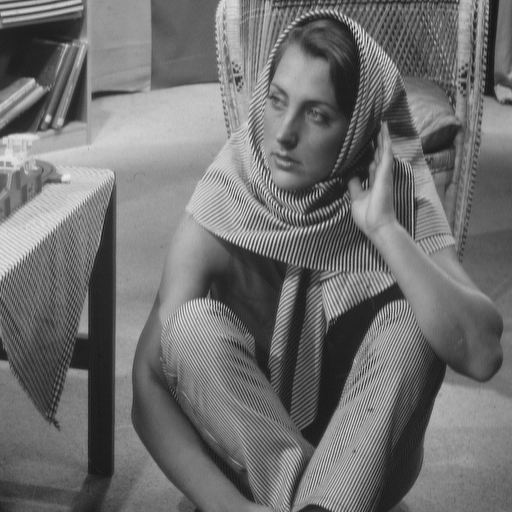
\includegraphics[width=3cm]{barb.png} & 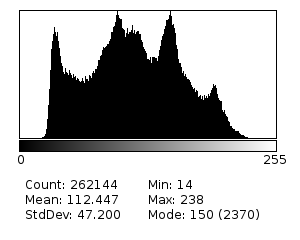
\includegraphics[width=3cm]{../histo/image/hist_barb.png} & 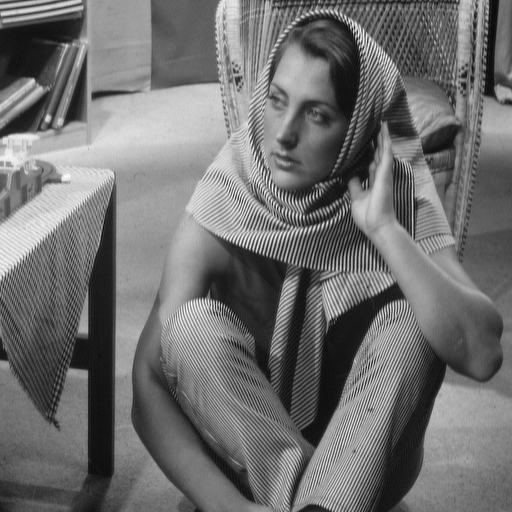
\includegraphics[width=3cm]{../res/barbQ1.png} & 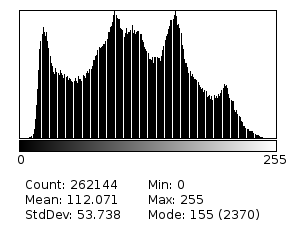
\includegraphics[width=3cm]{../histo/resultat/hist_barbQ1.png}\\
   \hline
   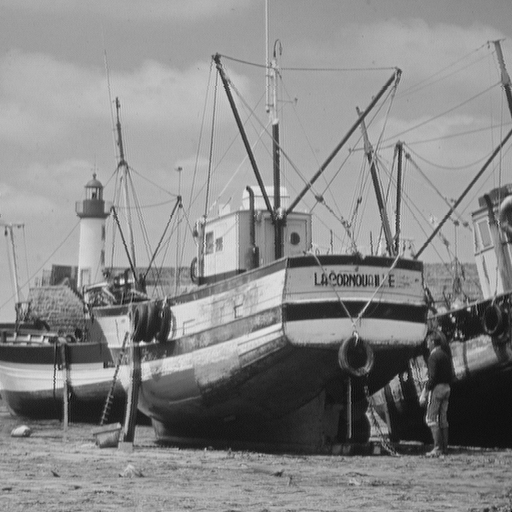
\includegraphics[width=3cm]{boat.png} & 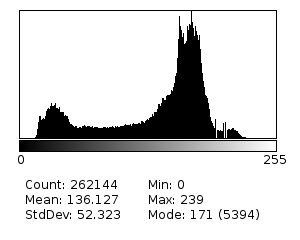
\includegraphics[width=3cm]{../histo/image/hist_boat.png} & 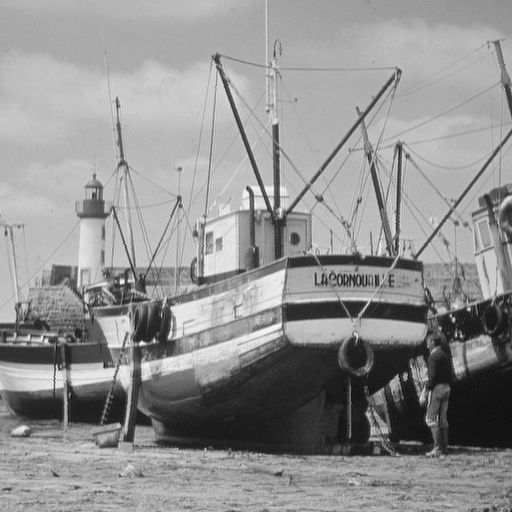
\includegraphics[width=3cm]{../res/boatQ1.png} & 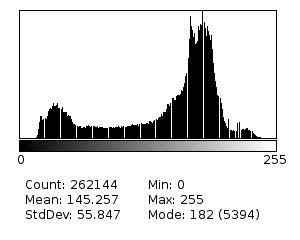
\includegraphics[width=3cm]{../histo/resultat/hist_boatQ1.png}\\
   \hline
   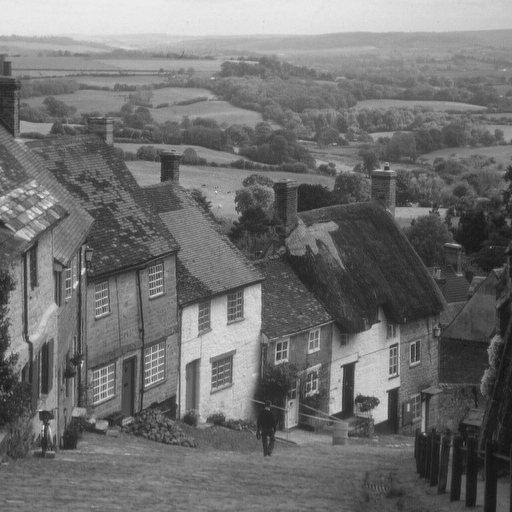
\includegraphics[width=3cm]{goldhill.png} & 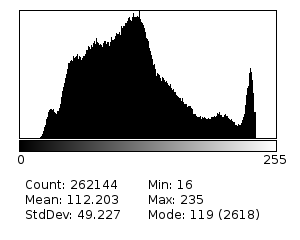
\includegraphics[width=3cm]{../histo/image/hist_goldhill.png} & 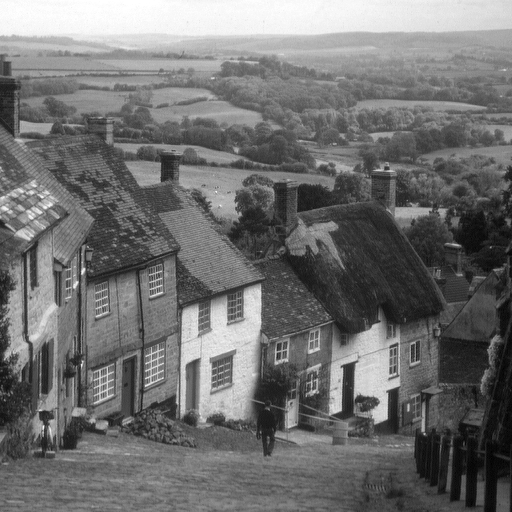
\includegraphics[width=3cm]{../res/goldhillQ1.png} & 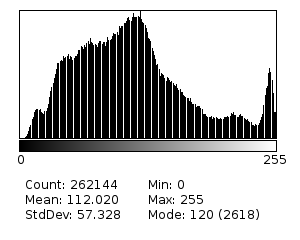
\includegraphics[width=3cm]{../histo/resultat/hist_goldhillQ1.png}\\
   \hline
  \end{tabular}
  
  \newpage
  
  \begin{tabular}{|c|c|c|c|} 
   \hline
   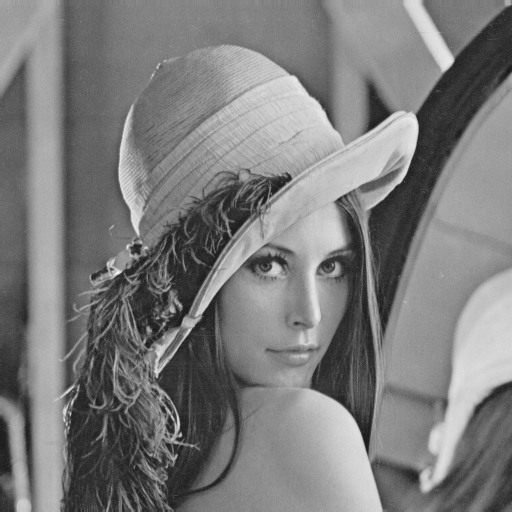
\includegraphics[width=3cm]{lena512.png} & 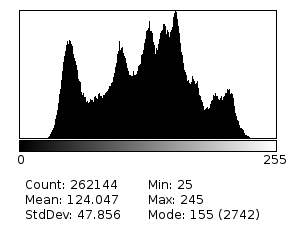
\includegraphics[width=3cm]{../histo/image/hist_lena512.png} & 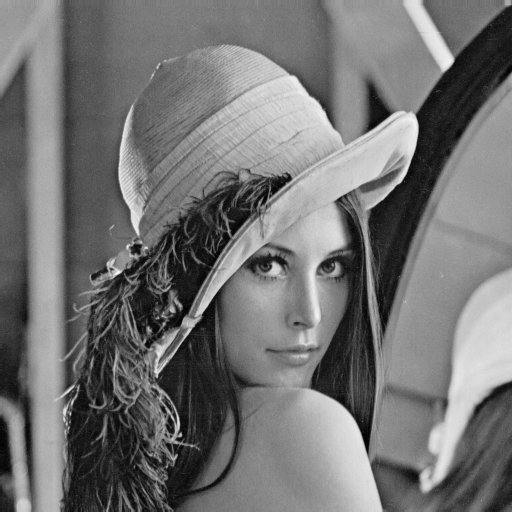
\includegraphics[width=3cm]{../res/lena512Q1.png} & 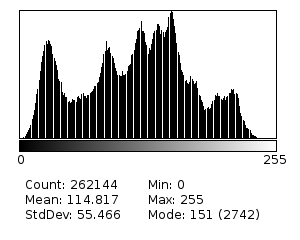
\includegraphics[width=3cm]{../histo/resultat/hist_lena512Q1.png}\\
   \hline
   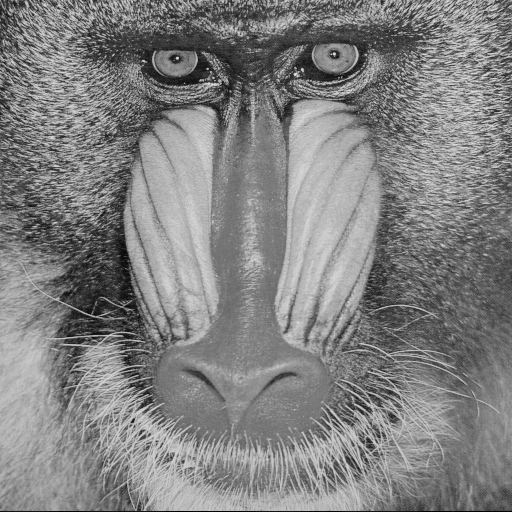
\includegraphics[width=3cm]{mandrill.png} & 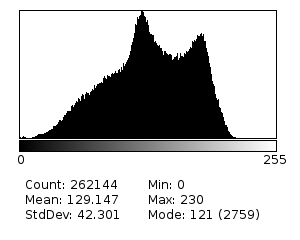
\includegraphics[width=3cm]{../histo/image/hist_mandrill.png} & 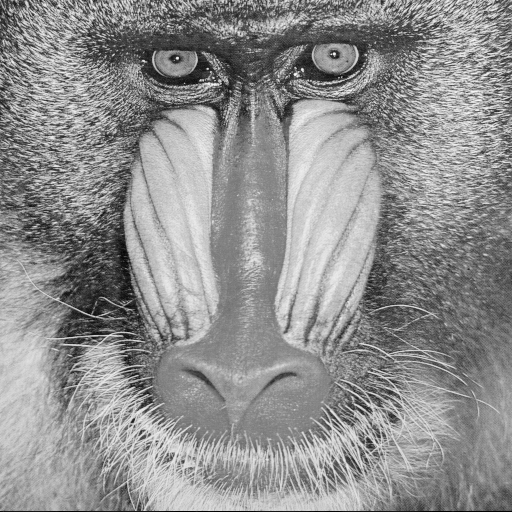
\includegraphics[width=3cm]{../res/mandrillQ1.png} & 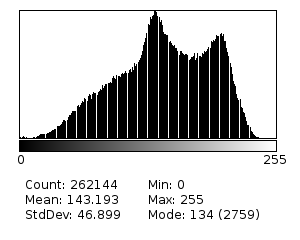
\includegraphics[width=3cm]{../histo/resultat/hist_mandrillQ1.png}\\
   \hline
   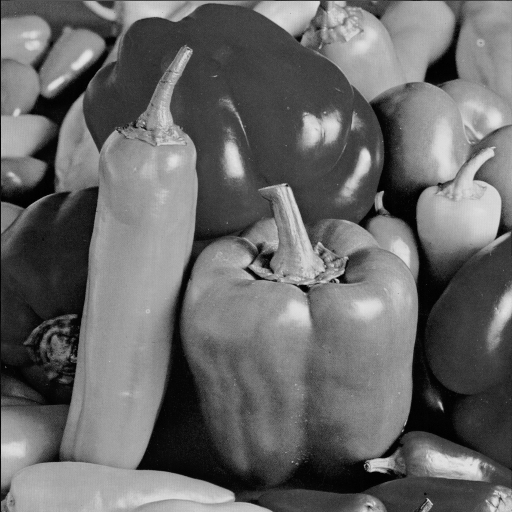
\includegraphics[width=3cm]{peppers.png} & 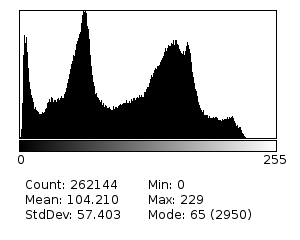
\includegraphics[width=3cm]{../histo/image/hist_peppers.png} & 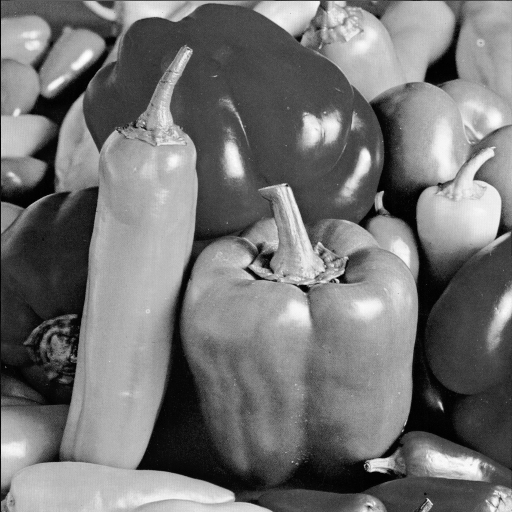
\includegraphics[width=3cm]{../res/peppersQ1.png} & 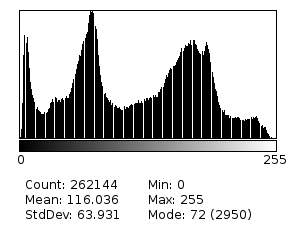
\includegraphics[width=3cm]{../histo/resultat/hist_peppersQ1.png}\\
   \hline
  \end{tabular}\\
  
  Sur ces résultats, nous pouvons voir que lorsque nous étendons l'histogramme de gris, le contraste de l'image augmente. Cela
  est d'autant plus visible lorque l'image originale n'avait aucun pixel dans le niveau 0.
  
  \section{Correction affine}
  Nous avons ensuite appliqué une correction affine du type $a+b.I(x,y)$ sur les images.
  Nous avons remarqué que plus la valeur de $a$ augmente, moins le contraste va être important.
  En effet, nous allons additionner une valeur constante à chaque pixel. Donc le nombre de pixel
  sombre va diminuer et le nombre de pixel dont la valeur va être supérieur à 255 va augmenter.
  Etant donné, qu'il n'y a pas plus de 256 niveaux de gris, le nombre de pixels blanc va augmenter
  et la différence entre les niveaux de gris minimum et maximum va se réduire.\\
  
  En revanche, la valeur de $b$ va intéragir sur la luminosité de l'image, plus la valeur sera grande,
  plus la luminosité sera importante.
  Etant donné que nous multiplions chaque pixel par une valeur constante, nous aurons de moins en moins
  de niveaux de gris dans l'image et le nombre de pixels dans les niveaux de gris très claire
  va augmenté.\\
  
  \begin{tabular}{|c|c|c|}
      \hline
      Image d'origine de la mandrill & 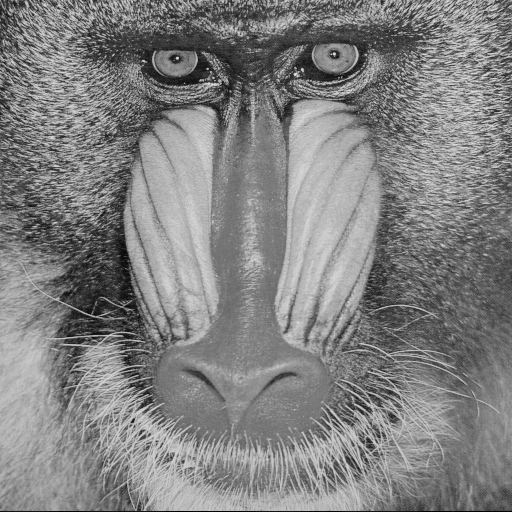
\includegraphics[width=3cm]{mandrill.png} & 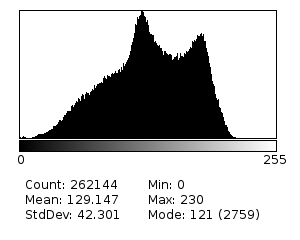
\includegraphics[width=4cm]{../histo/image/hist_mandrill.png}\\
      \hline
      Image avec a=50 et b=1 & 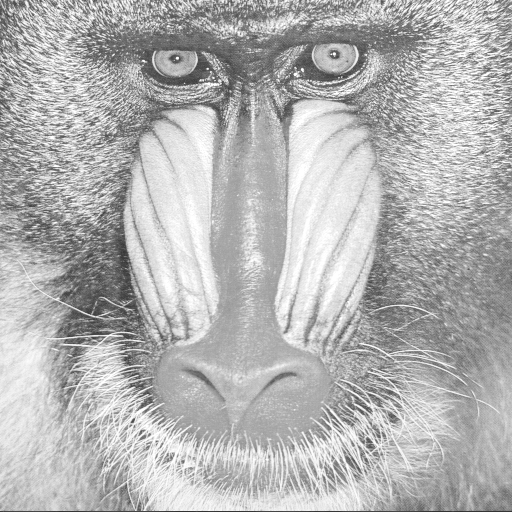
\includegraphics[width=3cm]{../res/mandrillQ2_50x1.png} & 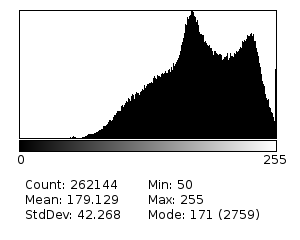
\includegraphics[width=4cm]{../histo/resultat/hist_mandrillQ2_50x1.png}\\
      \hline
      Image avec a=0 et b=2 & 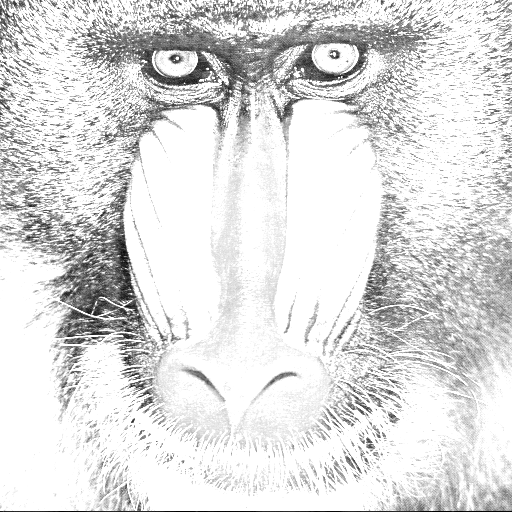
\includegraphics[width=3cm]{../res/mandrillQ2_0x2.png} & 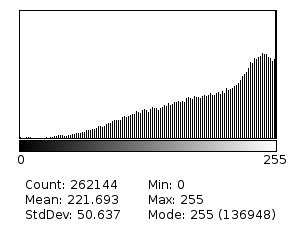
\includegraphics[width=4cm]{../histo/resultat/hist_mandrillQ2_0x2.png}\\
      \hline
  \end{tabular}
  
  
  \section{Egalisation d'histogramme}
  L'égalisation d'histrogramme est un procédé qui permet de mieu répartir les niveaux de gris sur une image.
  Pour pouvoir le calculer il nous faut d'abord récupérer l'histogramme cumulé. 
  Cette histogramme s'obtient en effectuant le calcul suivant : $hist(T)=hist(T)+hist(T-1)$. Nous obtenons donc
  un histogramme dont le nombre de pixel par niveau de gris augmente avec ce niveau. Ensuite, nous modifions la valeur de chaque pixel
  de l'image en utilisant une LUT. Lorsque nous allons modifier un pixel, nous reagardons dans une table de correspondance pour 
  connaitre la nouvelle valeur du pixel que nous voulons modifier. Pour cela nous utilisons la macro suivante :
  
  \begin{lstlisting}
       ratio = 255 / (W * H);

       for (j=0; j<H; j++) {
           for (i=0; i<W; i++) {
               p = getPixel(i, j);
               new = cumule[p];
               setPixel(i, j, new * ratio);
           }
       }
  \end{lstlisting}

  Ce qui nous donne les résultats suivant : \\
  
  \begin{tabular}{|c|c|c|c|}
   \hline
   image départ & histogramme & image égalisé & histogramme\\
   \hline
   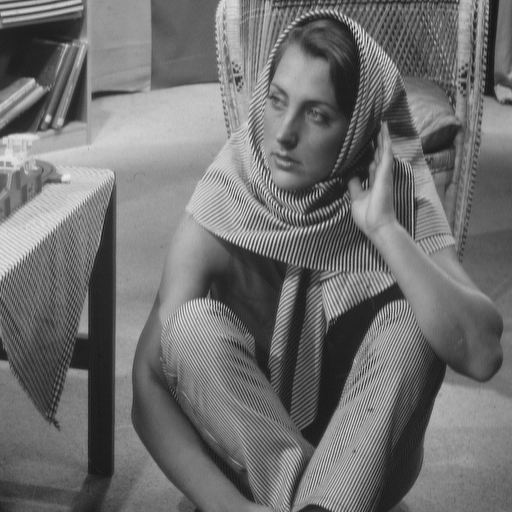
\includegraphics[width=3cm]{barb.png} & 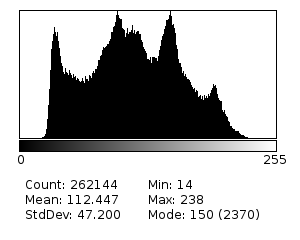
\includegraphics[width=3cm]{../histo/image/hist_barb.png} & 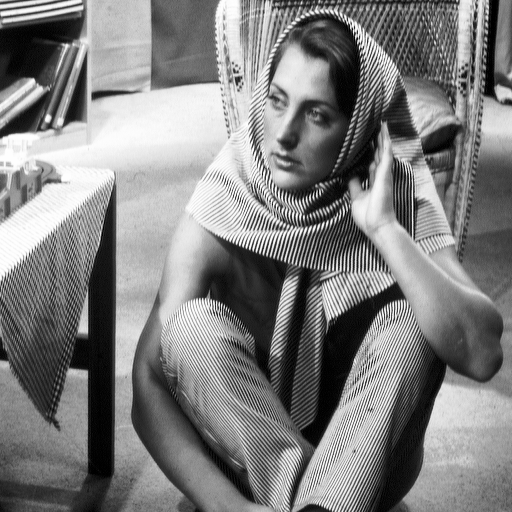
\includegraphics[width=3cm]{../res/barbQ3.png} & 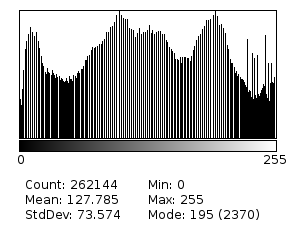
\includegraphics[width=3cm]{../histo/resultat/barbQ3.png}\\
   \hline
   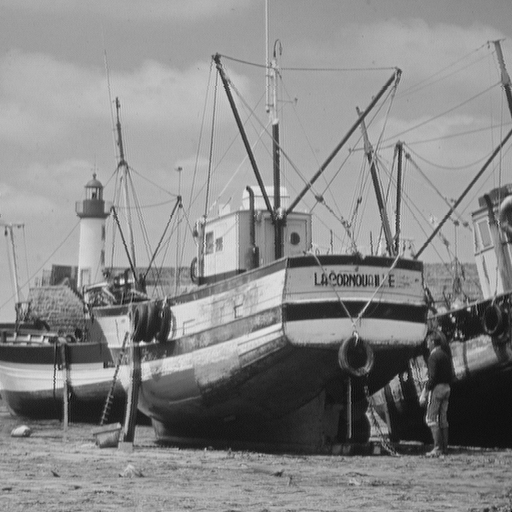
\includegraphics[width=3cm]{boat.png} & 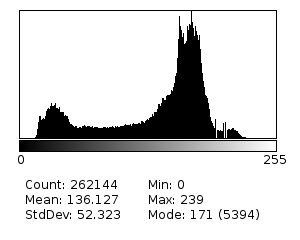
\includegraphics[width=3cm]{../histo/image/hist_boat.png} & 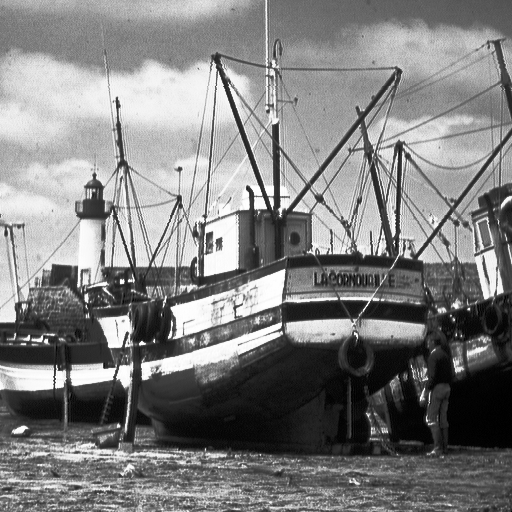
\includegraphics[width=3cm]{../res/boatQ3.png} & 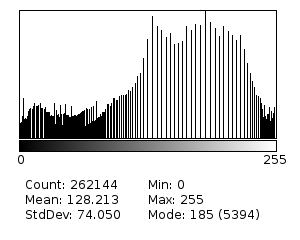
\includegraphics[width=3cm]{../histo/resultat/boatQ3.png}\\
   \hline
   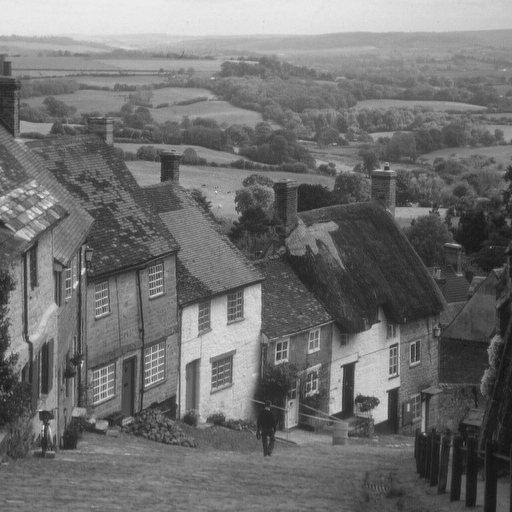
\includegraphics[width=3cm]{goldhill.png} & 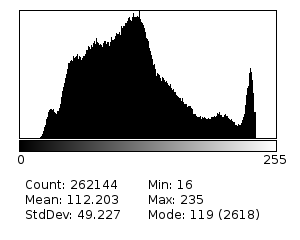
\includegraphics[width=3cm]{../histo/image/hist_goldhill.png} & 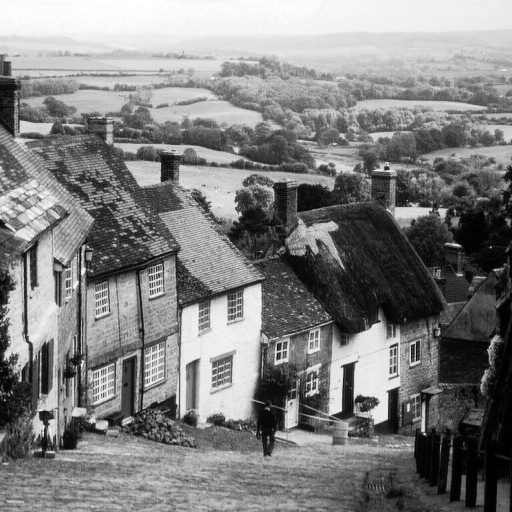
\includegraphics[width=3cm]{../res/goldhillQ3.png} & 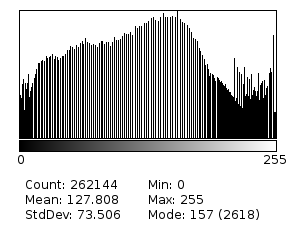
\includegraphics[width=3cm]{../histo/resultat/goldhillQ3.png}\\
   \hline
   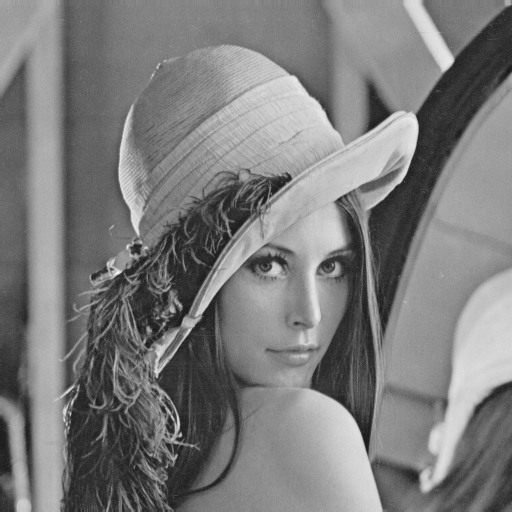
\includegraphics[width=3cm]{lena512.png} & 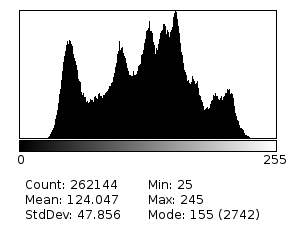
\includegraphics[width=3cm]{../histo/image/hist_lena512.png} & 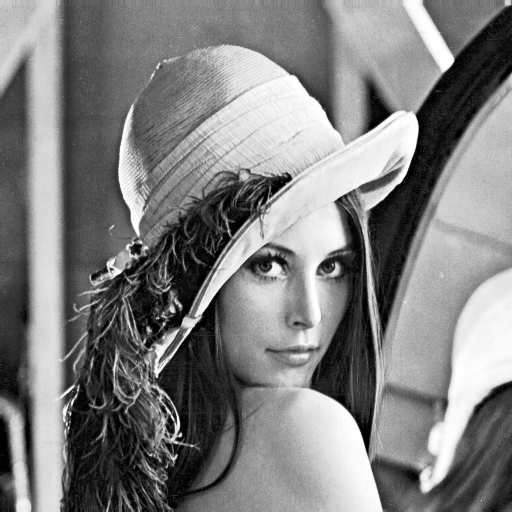
\includegraphics[width=3cm]{../res/lena512Q3.png} & 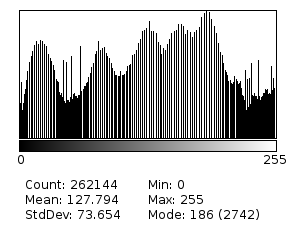
\includegraphics[width=3cm]{../histo/resultat/lena512Q3.png}\\
   \hline
   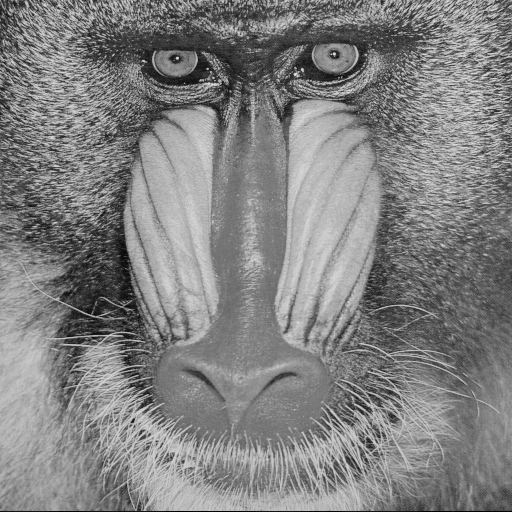
\includegraphics[width=3cm]{mandrill.png} & 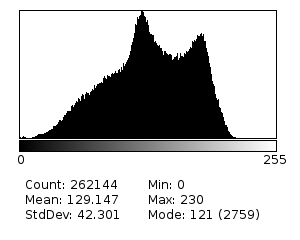
\includegraphics[width=3cm]{../histo/image/hist_mandrill.png} & 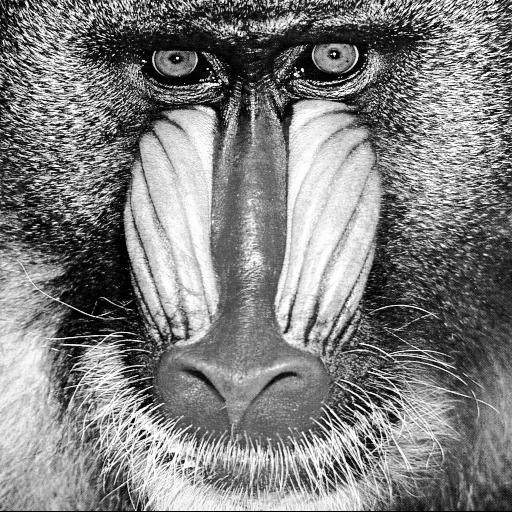
\includegraphics[width=3cm]{../res/mandrillQ3.png} & 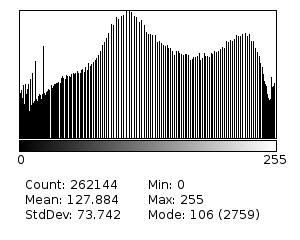
\includegraphics[width=3cm]{../histo/resultat/mandrillQ3.png}\\
   \hline
   \includegraphics[width=3cm]{peppers.png} & \includegraphics[width=3cm]{../histo/image/hist_peppers.png} & \includegraphics[width=3cm]{../res/peppersQ3.png} & \includegraphics[width=3cm]{../histo/resultat/peppersQ3.png}\\
   \hline
  \end{tabular}\\
  
  On peut voir que l'égalisation des histogramme n'est pas parfaite, que certain niveau gris ne sont pas utilisé et que d'autres 
  possèdent trop de valeur. Obtenir un histogramme parfaitement égalisé est très difficile, voir impossible.
  \section*{Conclusion}
  Lors de ce TP, nous avons pu voir plusieurs transformations d'histogramme et leur impacte sur l'image.
  \newpage
  
  \section*{Annexes}
  \begin{lstlisting}[caption=Macro d'extension d'histogramme]
  macro "setDynamiqueGray" {

    image = getImageID();

    W = getWidth();
    H = getHeight();

    min = 255;
    max = 0;

    for (j=0; j<H; j++) {
        for (i=0; i<W; i++) {

            p = getPixel(i,j);
            if ( min > p) {
                min = p;
            }

            if ( max < p) {
                max = p;
            }
         }
     }

     for (j=0; j<H; j++) {
         for (i=0; i<W; i++) {

             res = round(255 * ((getPixel(i,j) - min)/(max - min)));
             setPixel(i, j, res);
         }
     }
  }
  \end{lstlisting}
  
  \begin{lstlisting}[caption=Macro de la correction affine]
   macro "correction" {

      W = getWidth();
      H = getHeight();

      //contraste
      a = -100;
      //luminosite
      b = 2;

      for (j=0; j<H; j++) {
         for (i=0; i<W; i++) {

            res = a + b * getPixel(i,j);
            setPixel(i, j, res);
          }
      }
   }
  \end{lstlisting}

    
\end{document}  